\documentclass{scrartcl}

\usepackage[english]{babel}
\usepackage[hidelinks]{hyperref}
\usepackage{glossaries}
\usepackage{fancyvrb}
\usepackage{csquotes}
\usepackage{graphicx} 
\usepackage{color} 
\usepackage{transparent} 
\usepackage{import}
\usepackage{amssymb}
\usepackage{siunitx}
\usepackage{caption}
\usepackage{subcaption}
\usepackage{mathtools}
\usepackage[export]{adjustbox}[2011/08/13] 
\usepackage[hmargin=1.7in,vmargin=1.2in]{geometry}

\usepackage[comma,sort&compress]{natbib} 

\usepackage{epstopdf}
\usepackage{pdfpages}
\usepackage[version=3]{mhchem}
\usepackage{verbatim}
\usepackage{natbib}

\title{celltrack\\
	A 2D cell tracking algorithm (for DALES output)\\ \medskip
	v 0.2.beta}
\author{K. Lochbihler}

\begin{document}
	
\maketitle

\section{What is celltrack?}
celltrack is software that finds continuous cells in 2D fields and tracks them in time. The basic concept is inspired by \cite{moseley2013}. celltrack consists of several parts which are explained in detail in the following sections.

\subsection{Definitions}
The following two definitions are in accordance with \cite{moseley2013}.

\subsubsection*{Cell}
A cell is a continuous area of grid points which exceed a certain threshold. Two grid points are adjacent if their coordinates differ either in one x or one y step. Diagonal adjacency is not allowed.

\subsubsection*{Track}
A track is a time series of cells. Two cells are members of the same track if they (partly) overlap. The difference in time steps where the two cells occur is $(\pm)1$. This means that a track can not have more than one cell at each time step. 
\begin{figure}[h]
	\centering
	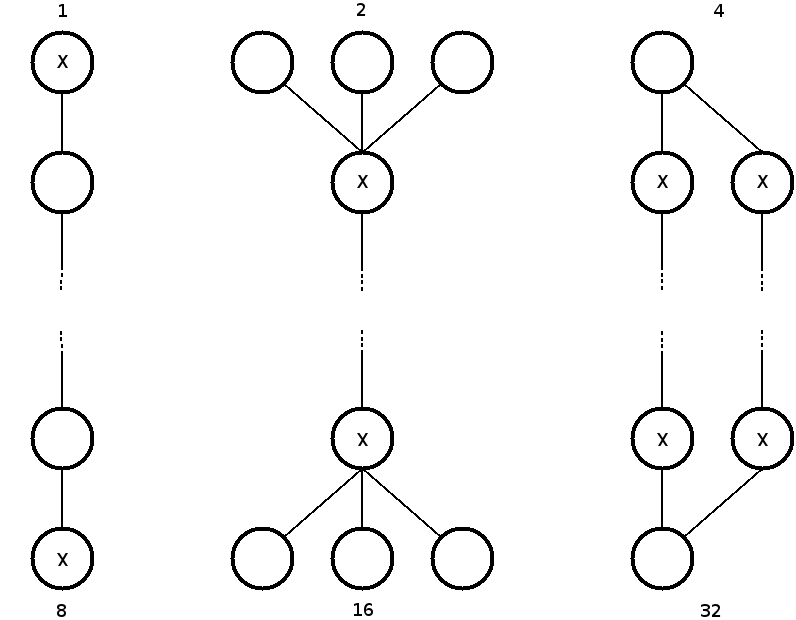
\includegraphics[width=.8\linewidth]{trackinitterm}
	\caption{The track taxonomy. There are 6 types of track initiation/termination. In total 9 combinations are possible. Adding up the numbers for initiation and termination a unique track type can be described. A X marks the responsible cell/beginning/end of track.}
	\label{trackinitterm}
\end{figure}
A track is initiated by one of the following circumstances:
\begin{itemize}
	\item a cell has no overlap with cells from the previous time step
	\item a cell overlaps with more than one cell from the previous time step
	\item in both cases the cell must not overlap with more than one cell in the next time step
\end{itemize}
Cells which have overlaps with only one cell from the previous and next time step need to be distinguished further:
\begin{itemize}
	\item if the backward link cell splits, a new track is splitting from an existing one
	\item if not, this cell is in the interior of a track.
\end{itemize}
 A cell with the following properties ends a track:
\begin{itemize}
	\item there is no overlap with cells from the next time step
	\item merges with other cells in the next time step
	\item splits into several cells in the next time step
\end{itemize}
The structure of these 6 different ways of initiating and terminating a track are illustrated in figure \ref{trackinitterm}. Each possibility has a number. Adding up the numbers for track initiation and termination type a unique identifier for the track type can be derived. A track with type 33 for example has a beginning and ending of 1 and 32. 

\subsection{The clustering algorithm}
This part does the cell detection. Therefore celltrack iterates the two spatial dimensions to find continuous areas and assign an unique (integer) ID to them. The following decisions are made for each grid point with a value that exceeds the threshold:
\begin{itemize}
	\item no adjacent grid point which already has an ID: assign new ID
	\item one adjacent grid point which already has an ID: use this ID
	\item two or more adjacent grid points which already have  IDs:
	\begin{itemize}
		\item these grid points have the same ID: use this ID
		\item different IDs: use the lowest ID for all grid points
	\end{itemize}
\end{itemize}
This step is repeated for every time step. At the end of this step all detected cells have unique IDs. This procedure leads to the fact that a cell A with a higher (lower) ID than cell B occurs at the same time step or later (earlier).

\subsection{The linking}
In this part all cells are checked for forward and backward links (one time step) with other cells. The results are stored in a logical matrix which has the size $n * n$, where n is the number of detected cells. Each row/column belongs to a particular cell ID. For an example, see figure \ref{links}: If the linking matrix is true at row 4 and column 7, the cell with ID 4 has a forward link with cell 7.

The logical link matrix makes it easy to check for overlaps between two cells any time later.

\subsection{The tracking algorithm}
Using the logical link matrix the tracking part is quite simple. For each row (which corresponds to a specific ID) the algorithm checks whether there are cells with higher and lower IDs that are linked i.e. the link matrix is TRUE at this address. Counting these the number of forward and backwards links in time can be determined. Based on this information and using the link matrix it is known which IDs initiate a track according to the definition given above. If an ID is at the beginning of a track the algorithm changes to the corresponding row in the link matrix and searches for forward links to cells in the next time step. If there is such a connection the algorithm changes to the corresponding row. This step is repeated until the conditions for terminating a track are met.
\begin{figure}[h]
	\centering
	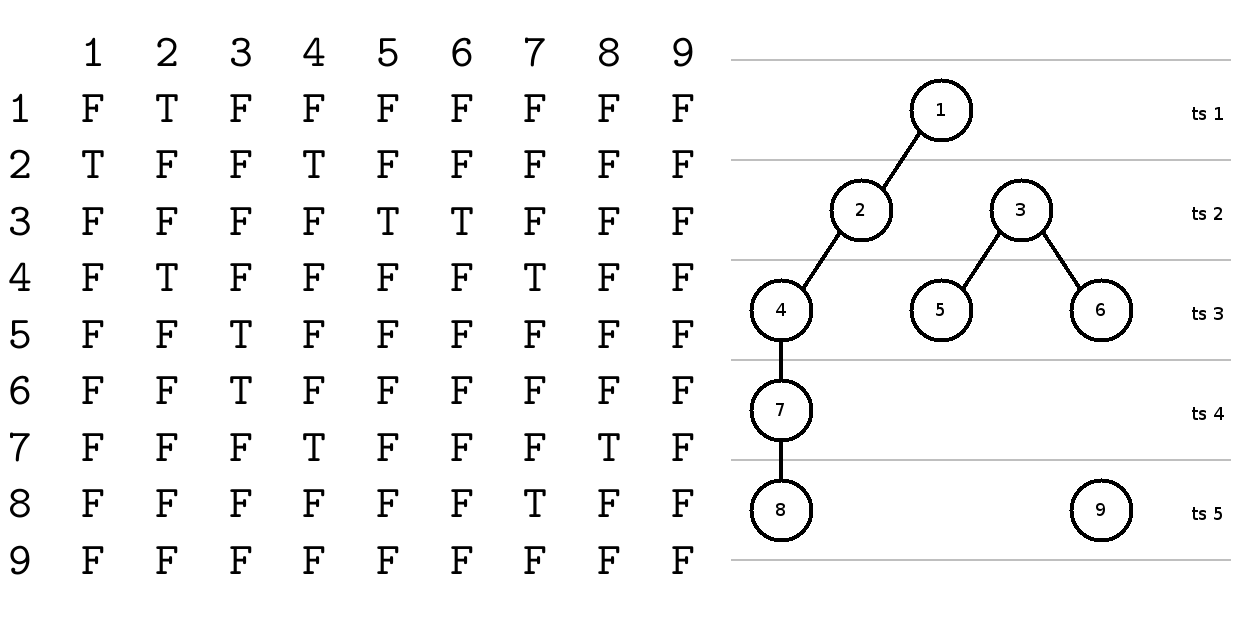
\includegraphics[width=.8\linewidth]{links}
	\caption{Example logical link matrix with IDs and the corresponding linking tree.}
	\label{links}
\end{figure}
Figure \ref{links} shows a basic example of a link matrix. Based on this one can easily generate the corresponding topology tree which shows all cells and their relationships.

\subsection{Meta tracks and mainstream detection}
With increasing length and/or cell sizes it becomes more and more likely that a track ends with a split or merge into/with other track(s). Although, celltrack puts those snippets into the same category as type 9 tracks one could argue that a combination of such related segments forms a complete track as well. For this reason the term \textit{meta track} is introduced. Essentially, a meta track is a group of tracks of different types which are connected directly or through a chain of an arbitrary number of tracks.
\begin{figure}[h]
	\centering
	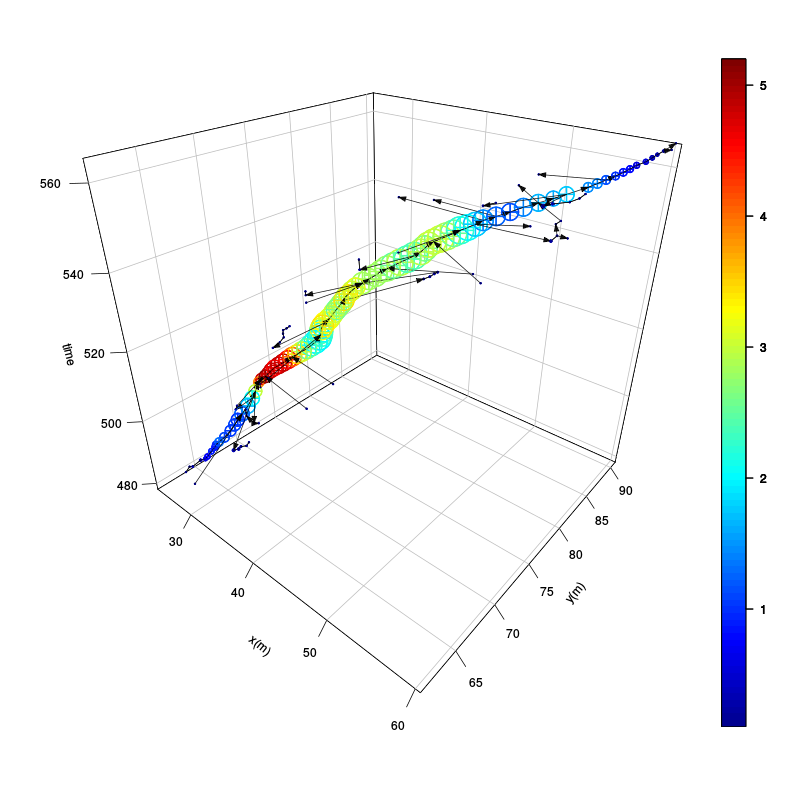
\includegraphics[width=.8\linewidth]{scatter3D_meta_2}
	\caption{A rather abstract visualization of a meta track. Colors indicate the peak rainfall intensity of a cell (mm/10min). The Size of the symbols is proportional to cell area. The arrows show the direction of a connection between two tracks. The time axis is in minutes.}
	\label{meta_track}
\end{figure}
Figure \ref{meta_track} shows an example for a fairly large meta track. It consists of 52 tracks and has a lifetime of 88 minutes. Apart from a dominant \textit{mainstream} there are lots of small tributaries and tracks that split away. It is obvious that they have low cell sizes as well as intensities.

To separate the dominant mainstream from dead ends and tributaries, celltrack uses a metaheuristic approach called ant colony optimization (ACO) \citep{Dor1992:thesis}. \cite{DorSta2004:book} give an overview about theory and application of different ACO methods. ACO is inspired by the behavior of foraging ants which are able to find a minimum cost (length) path from a nest to a source of nurture through indirect communication. This is accomplished by modifications of the environment in form of pheromone deposit. To apply this principle to the problem of mainstream detection in meta tracks we have to rise our point of view to a more abstract level. As well as the possible paths from a nest to a source of nurture, a meta track can be seen as a network consisting of nodes and arcs. Using this notation a meta track can be translated into a construction graph where tracks are arcs and the connections between tracks are the nodes.
\begin{figure}[h]
	\centering
	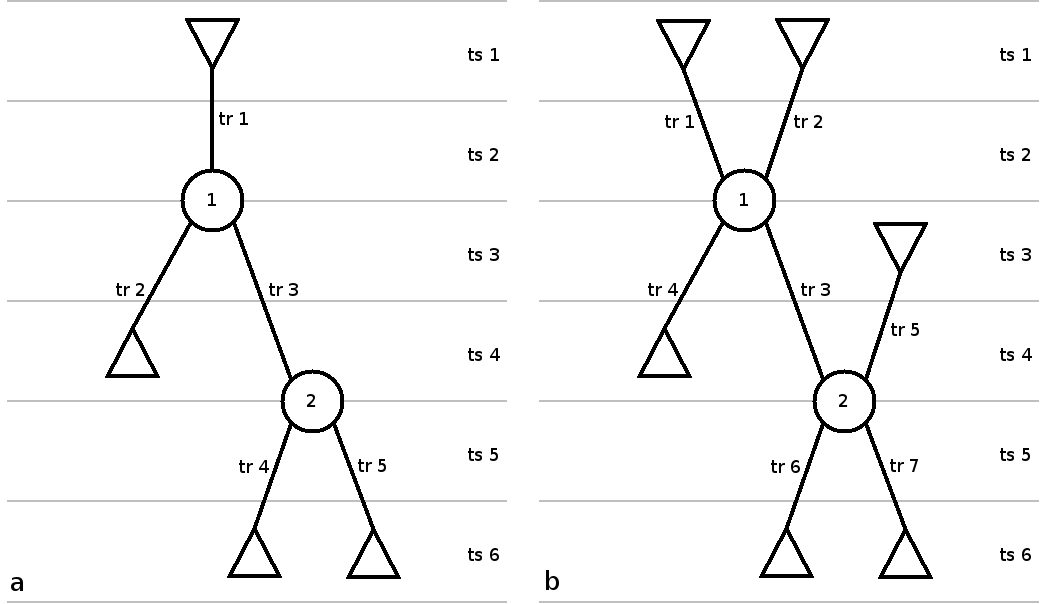
\includegraphics[width=.8\linewidth]{construction_graphs}
	\caption{Two simple examples for a construction graph of a meta track. Circles represent nodes; lines show tracks. Triangles denote points of initiation and termination.}
	\label{meta_track_con}
\end{figure}

A very simple example for a construction graph of a meta track is depicted in figure \ref{meta_track_con}a. It is clearly visible that there are three possible paths following the tracks
\begin{enumerate}
	\item tr1 - tr2
	\item tr1 - tr3 - tr4	
	\item tr1 - tr3 - tr5.
\end{enumerate}
To rank these candidate solutions by quality, celltrack calculates the average cost of a path by $\overline{C}=\frac{1}{m}\sum_{k=1}^{m}{c_{ij}^k}$ with the number of nodes in this path ($m$) and the difference in peak intensities ($c_{ij}^k$) between the last cell of track $i$ and first cell of track $j$ at the $k\textendash th$ node of this path. This defines the mainstream as the one path of arbitrary length (time/tracks) with the on average smoothest transitions between connected tracks. Concerning the example in figure \ref{meta_track_con}a it is fairly easy to compute the cost for all paths and detect the one with the lowest cost value as mainstream. But, switching to the example in figure \ref{meta_track_con}b makes things more complicated. Although only two tracks were added to the construction graph, the number of candidate solutions increases from three to eight. But still, it is feasible to compute all solutions and chose the best. However, the assumption is that the number of possible solutions increases exponentially with the complexity of a meta track. Thus, it is necessary to introduce an optimization algorithm. ACO algorithms can reduce the computation time to find a reasonable solution to combinatorial problems. celltrack incorporates a simplified version of an ACO algorithm \citep{DorSta2004:book} to find a mainstream of a meta track at low computational cost. It consists of the following steps
\begin{enumerate}
	\item initialize the pheromone values of all arcs by $\tau_{ij}=m/\overline{C^{nn}}$, where $\overline{C^{nn}}$ is the cost value of a nearest-neighbor path of length $m$ (number of nodes) starting at a random initiation point
	\item a certain number of artificial ants construct candidate solutions
	\item compute cost values for each ants path
	\item lower pheromone trails of all arcs using $\vartriangle \tau_{ij}^{k}=(1-\rho)\tau_{ij}^{k}$
	\item increase pheromone trails by $\vartriangle \tau_{ij}^k=1/\overline{C}$ for each ants path
	\item After repeating steps 2 to 5 certain times, construct a nearest-neighbor path using the inverse pheromone values as a distance measure starting at the initiation point with the highest pheromone value.
\end{enumerate}
\begin{figure}[h]
	\centering
	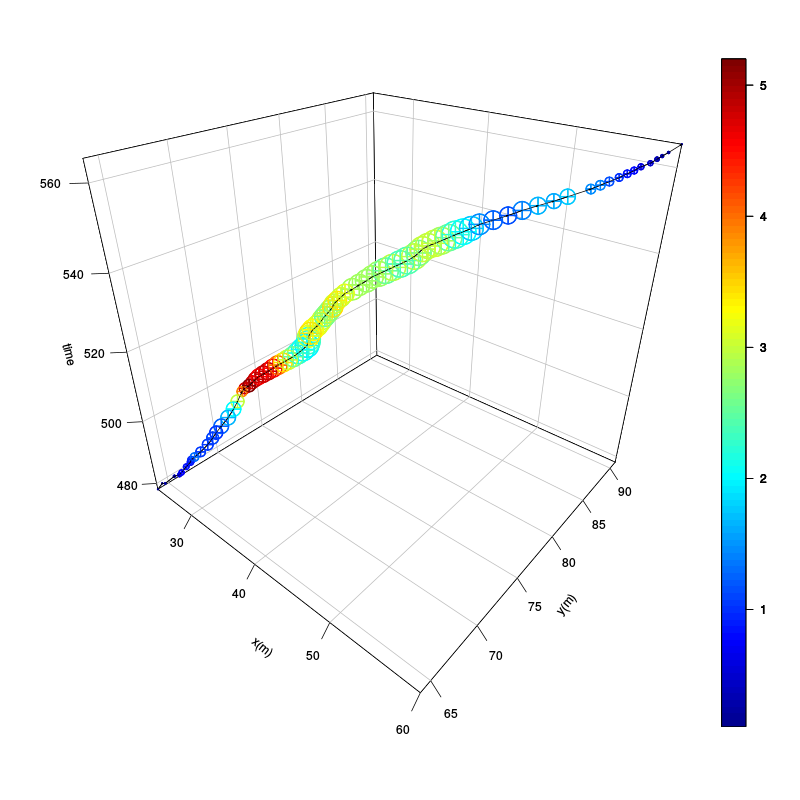
\includegraphics[width=.8\linewidth]{scatter3D_meta_mainstream_2}
	\caption{The mainstream of the meta track shown in figure \ref{meta_track}; as detected by the ACO algorithm.}
	\label{meta_track_mainstr}
\end{figure}

Step 2 needs further explanation; this is how an ant constructs a solution: 
\begin{enumerate}
	\item randomly select an initiation/termination point
	\item walk to the next node
    \item calculate the probabilities for all possible choices at this node with $p_{ij}=\frac{\tau_{ij}^\alpha \eta_{ij}^\beta}{\sum_{l\in N_i} {\tau_{il}^\alpha \eta_{il}^\beta}}$ with $j \in N_i$. $N_i$ is the group of possible tracks to follow when coming from track $i$, $\eta_{ij}=1/c_{ij}$ is the heuristic value. $\alpha$ and $\beta$ determine the influence of the pheromone and heuristic value. Decide with these probabilities using a random number.
    \item repeat steps 2 and 3 until a termination/initiation point is reached.
\end{enumerate}
The reason for randomly switching between a forward and backward in time direction is that only randomly starting at initiation points leads to equal probabilities  because this decision is not based on the formula of step 3.

Figure \ref{meta_track_mainstr} shows the mainstream of the meta track which was previously depicted in figure \ref{meta_track}.  

\subsection{The other stuff}
Apart from clustering and tracking there are also routines that calculate cell and track statistics. For this purpose, celltrack uses values from the input file. For detailed descriptions see section \ref{sec:output}.

\section{Building from source}
\subsection{Dependencies}
The following dependencies are mandatory to compile and run celltrack:
%To read netCDF and grib data celltrack uses the cdi library which is the input/output part of cdo. cdi has to be compiled with netCDF support. Thus, the netCDF library 
\begin{itemize}
	\item cdi
	\item all dependencies of cdi, e.g. netCDF, grib\_api
\end{itemize}

\subsection{configure and make}
Beginning with version 0.2.beta cmake is used to configure and create the Makefiles. The following commands should do the job (run within the celltrack directory):
\begin{verbatim}
mkdir build
cd build
cmake ..
make
\end{verbatim}
If you want to install the celltrack binary run
\begin{verbatim}
make install
\end{verbatim}
Remember that this most likely requires root privileges. For a custum path run cmake with 
\begin{verbatim}
cmake .. -DCMAKE_INSTALL_PREFIX=/custom/path
\end{verbatim}
If the cdi include and library are not in your environment variables you can run cmake with the following options
\begin{verbatim}
cmake .. -DCDI_INCLUDE=/path/to/include/dir/ \
  -DCDI_LIB=/path/to/lib/dir/libcdi.so
\end{verbatim}
or change the values of the according keys in CMakeCache.txt in the build directory.

Another way to tell cmake where to find the cdi include and library is setting the environment variables CDI\_INCLUDE\_PATH and CDI\_LIB\_PATH. In bash this can be done running
\begin{verbatim}
export CDI_INCLUDE_PATH=/path/to/include/dir/
export CDI_LIB_PATH=/path/to/lib/dir/
\end{verbatim}
then run
\begin{verbatim}
cmake ..
make
\end{verbatim}
To run celltrack the path to the cdi library must be in the environment, for example using the LD\_LIBRARY\_PATH variable on Linux platforms.

\section{Usage}
\begin{verbatim}
celltrack -i <filename> -var <int> -lev <int> -thres <float> \
          -nants <int> -nruns <int> -rho <float> \
          -rseed <int> -o <file> -lout -v -h
\end{verbatim}

\subsubsection*{Example}
\begin{verbatim}
celltrack -i surfprec.nc -var 0 -lev 0 -thres 0.5
\end{verbatim}

\subsubsection*{Options}
\begin{labeling}{-rseed }
	\item[-i] Input file name.
	\item[-var] NetCDF/grib variable ID. Default is 0.
	\item[-lev] NetCDF/grib level ID. Default is 0 i.e. the first variable.
	\item[-thres] All grid points with values greater than this are considered. Default is 0.
	\item[-nants] Number of agents for mainstream detection. Default is 15.
	\item[-nruns] Number of iterations for mainstream detection. Default is 300.
	\item[-rho] Pheromone evaporation. Default is 0.5.
	\item[-rseed] If set, the random number generator will use this seed.
	\item[-o] Output file name. Default is 'cells.nc'.
    \item[-lout] Write the truncated logical links matrix to file cell\_links.txt.
	\item[-v] Verbose output to stdout. Use with caution! Massively slows down code execution!
	\item[-h] Show help.
\end{labeling}

\section{Input}
celltrack should be able to read all file formats which are supported by cdi. However, currently only netCDF has been tested.
celltrack expects 3D data:
\begin{enumerate}
	\item x axis
	\item y axis
    \item time axis
\end{enumerate}

\section{Output}
\label{sec:output}

\subsection{The cells files}
\subsubsection{cells.nc}
This is the first file celltrack will create. It has the same structure as the input file and contains the unique cell IDs. The default file format is netCDF.

\subsubsection{cell\_stats.txt}
This file contains some simple statistics about the detected cells. The columns are:
\begin{labeling}{wclcmassX}
	\item[clID] The cell ID.
	\item[tsclID] The time step this cell occurs.
	\item[clarea] The area in unit grid points.
	\item[clcmassX] The x coordinate of the center of mass.
	\item[clcmassY] The y coordinate of the center of mass.
	\item[wclcmassX] The x coordinate of the weighted center of mass.
	\item[wclcmassY] The y coordinate of the weighted center of mass.
	\item[peakVal] The maximum value.
	\item[avVal] The average value.
	\item[bound] TRUE if the cell touches the boundaries.
\end{labeling}

\subsection{The links files}
\subsubsection{cell\_links.txt}
This file is rather intended for development and debugging. It contains the truncated logical link matrix. The rows represent cells which are the same like in cell\_stats.txt. Because the matrix is truncated each row contains only cells which appear at the same, one before and after time step of the corresponding row/cell. The first column mentions the point of truncation. The second column names the first ID in each row. With this information the complete $n*n$ matrix can be reconstructed. The third column contains the column number of each row/cell in the link matrix.

\subsubsection{links\_stats.txt}
This file contains the number of forward and backward links for each cell. The columns:
\begin{labeling}{clID}
	\item[clID] The cell ID.
	\item[nbw] The number of backward links.
	\item[nfw] The number of forward links.

\end{labeling}

\subsection{The tracks files}
\subsubsection{tracks\_all.txt / tracks\_clean.txt}
These files list tracks with an object-oriented structure. The first line of each block (beginning with \#\#\#) gives important information about the track. The first integer is the track ID. Then, a logical value tells if the track touches the boundaries of the domain. The last number is the track type as explained in figure \ref{trackinitterm}. Following the header, all cells of a track are listed. The only column is:
\begin{labeling}{clcmassX}
	\item[clID] The cell ID.
\end{labeling}
The difference between the two files is that tracks\_clean.txt only lists tracks which are of type 9 and do not touch the boundaries during their lifetime. 

\subsubsection{tracks\_all\_stats.txt / tracks\_clean\_stats.txt}
The structure of this files is the same as in tracks\_all.txt / tracks\_clean.txt. However, there are some additional columns:
\begin{labeling}{peakVal}
	\item[clID] The cell ID.
	\item[tsclID] The time step this cell occurs.
	\item[clarea] The area in unit grid points.
	\item[clcmassX] The x coordinate of the center of mass.
	\item[clcmassY] The y coordinate of the center of mass.
	\item[wclcmassX] The x coordinate of the weighted center of mass.
	\item[wclcmassY] The y coordinate of the weighted center of mass.
	\item[peakVal] The maximum value.
	\item[avVal] The average value.
	\item[bound] TRUE if the cell touches the boundaries.
\end{labeling}
The difference between the two files is that tracks\_clean\_stats.txt only lists tracks which are of type 9 and do not touch the boundaries during their lifetime.

\subsubsection{tracks\_all\_summary.txt / tracks\_clean\_summary.txt}
The summary files contain overall statistics for all tracks/tracks of type 9 which do not touch the boundaries. The columns represent:
\begin{labeling}{pValtime}
	\item[trackID] The cell ID.
	\item[trType] The track type according to figure \ref{trackinitterm}.
	\item[peakVal] The maximum value.
	\item[pValtime] The time step of the maximum value.
	\item[avVal] The average value.	
	\item[start] The time step at which a track starts.
	\item[dur] The duration/life time.
\end{labeling}

\newpage
\bibliographystyle{apalike}
\bibliography{celltrack_doc}
\end{document}
